% ===================================================================
% Supplementary Material --- v2 diffusion-based inverse-RG model
% Paste into your paper where the appendix/supplementary section goes.
% Assumes: \usepackage{graphicx}, \usepackage{amsmath}, \usepackage{amssymb},
%          \usepackage{booktabs}
% Images expected at figures/01_ladder_drift.png ... figures/27_program_optimum.png
% ===================================================================

\section{Supplementary Material --- v2 Model}
\label{sec:appendix-v2}

This appendix documents the v2 checkpoint of the diffusion-based inverse-RG
sampler for 2D compact U(1) lattice gauge theory. It addresses five
questions: (1) does the generated ensemble match exact results, inside and
far outside the training range; (2) how does the sampler compare, in
wall-clock cost and correctness, against the strongest classical baseline we
could construct (instanton-update HMC, whose global $Q$-hop is the
volume-independent uniform $Q$-shift move); (3) what a diffusion-generated
configuration buys as an HMC starting point; (4) what an
exact-likelihood diagnostic honestly says about the model as an
importance-sampling proposal; and (5) how far sampling-time tuning and
likelihood-aware fine-tuning can close that importance-sampling gap ---
including which standard remedies fail, and why.

\subsection{What this appendix establishes}
\label{sec:appendix-v2-contributions}

The sampler is the \emph{instrument}, not the claim. Learned coarse-to-fine
maps for lattice field theory are an established line --- inverse-RG
upscaling of configurations, RG-inspired coarse$\to$fine flows, diffusion
models for gauge theory, and the classical multiscale-thermalization
algorithms they descend from. What that line has not done is ask whether the
generated ensemble is the Boltzmann distribution: it is validated on
observables --- critical exponents, Wilson loops, topological
susceptibility. Incorporating numerical exactness into inverse-RG methods is
named as open work in that literature.

This appendix answers it, for a sampler that passes conventional validation
by a wide margin. Four results:

\begin{enumerate}
  \item \textbf{A way to measure distributional correctness when ESS is
    uninformative} (Sec.~\ref{sec:appendix-v2-measuring}). Self-normalized
    ESS is the usual check and it degenerates here --- ${\rm ESS}/N$ sits at
    exactly $1/N$, the estimator's floor rather than a measurement, and
    cannot distinguish a 10-nat gap from a 100-nat one. The free-energy
    identity converts the same weights into a \emph{direct} KL readout in
    nats/site that stays informative after ESS has bottomed out.
  \item \textbf{The measurement.} ${\approx}0.88$ nats/site at $L = 16$,
    $\beta = 55$ and 1.02 at $L = 32$, $\beta = 218.6$ --- i.e.\ 448 and
    2098 nats per configuration.
  \item \textbf{The dissociation, and where it becomes visible}
    (Sec.~\ref{sec:appendix-v2-sharpness}). The same ensembles reproduce the
    plaquette to two parts in $10^4$. The two facts are consistent because
    low-order gauge-invariant observables are a very low-dimensional
    projection of a $2L^2$-dimensional measure --- and the residual
    \emph{is} detectable once one looks at extended observables, where the
    $z$-dispersion grows monotonically with loop area. Short-distance
    agreement does not certify the measure.
  \item \textbf{A falsification chain rather than a shrug.} Six
    interventions --- sampling-time knobs, maximum-likelihood fine-tuning at
    two capacities, single- and multi-case reverse-KL, capacity/data
    scaling, per-level SMC, and surrogate-bridge AIS --- converged, with a
    mechanism identified for each. The one control that could have explained
    the gap away, an exactly-matched action arm, eliminates it
    (Table~\ref{tab:matching-residual}): the gap is fine-side model error.
\end{enumerate}

The practical consequence, validated by
Figs.~\ref{fig:headtohead}--\ref{fig:entry-cost} and \ref{fig:three-way}:
correctness for this class of sampler has to come from Markov-chain
machinery wrapped around the proposal --- seeded chains, Metropolis tails,
structural sector imposition --- not from the proposal's own density. A
reporting protocol is given in Sec.~\ref{sec:appendix-v2-protocol}.

\subsection{Methodology}
\label{sec:appendix-v2-methods}

\paragraph{The model.} A gauge-covariant score network (invariant
plaquette/rectangle inputs, plaquette-curl output head, per-site channel
normalization) is trained by denoising score matching on wrapped link angles
$\theta \in (-\pi,\pi]$, conditioned on the $2\times 2$-blocked coarse
field, over continuous log-uniform couplings $\beta \in [1, 60]$ at
$L = 8, 16, 32$. Generation runs the reverse process as one inverse-RG step
(coarse $\beta_c$ at $L$ $\to$ fine $\beta_f$ at $2L$, matched so the
blocked fine theory reproduces the coarse one). Relative to the previous
(v6) checkpoint, v2 adds: exact-symmetry data augmentation ($90^\circ$
rotations, reflections, and charge conjugation $\theta \to -\theta$, which
enforces $P(Q) = P(-Q)$ statistically); oversampling of small noise levels
at high $\beta$ (targeting the $\sigma$-region that resolves the narrow
high-$\beta$ link distributions); a per-site normalization with no
lattice-size dependence; a global coarse-FiLM channel carrying the coarse
winding sum $2\pi Q/V$ to every layer; and a $\beta$-gated exact-score
blend (analytic noised-Wilson score as $\sigma \to 0$, gated off below
$\beta \approx 5$).

\paragraph{Honesty conventions.} All topology results use the strict
setting: rethermalization performs \emph{no} topological (instanton-hop)
updates, so the model plus the deterministic coarse-charge transport must
carry the sector --- rethermalization cannot manufacture topology. Raw
(pre-enforcement) topology metrics are quoted where model transport itself
is at issue. Error bars are per-chain time averages (never pooled across
time $\times$ chain) for HMC series, and per-config SEM for generated
ensembles; $z$-scores are against exact character-expansion values. Two
independent seeds were run for the out-of-sample tracks; all seed-2 results
confirmed seed-1 within statistics.

\paragraph{Sector modes.} The pipeline exposes two topological-sector
treatments. \emph{Transport} (the strict default above): the fine sector is
the coarse configuration's sector, carried deterministically by the smooth
instanton shift --- final $P(Q)$ is the coarse base's empirical histogram,
so this mode measures what the model itself carries, but it cannot retarget
topology when the requested $\beta_f$ is not the base's matched coupling.
\emph{Exact-sector} (production): the coarse base is first
charge-conjugation symmetrized (C-antithetic: half the batch is mapped
$\theta \to -\theta$, exactly measure-preserving, enforcing $P(Q) = P(-Q)$
at finite sample size), and each configuration's sector is then drawn from
the exact finite-volume $P(Q)$ at the \emph{target} coupling and imposed by
the same instanton shift. Sector statistics are then correct by construction
at any target --- the honest successor to hop-in-rethermalization, and this
pipeline's analogue of $Q$-shift sector reconstruction. Wilson observables
are statistically identical in the two modes (mean plaquette $|z|$
\emph{vs the HMC reference} 1.77 vs 1.74 over 38 cases; against the exact
character expansion, the convention used everywhere else here, 1.06 vs
1.08).

\paragraph{Statistical baseline.} Under these conventions the v2 checkpoint
matches exact results across 38 study cases from $\beta_f = 1.49$ to
$872.8$ ($15\times$ the training maximum) and volumes to $L = 128$
($16\times$ the largest training area, $64\times$ the smallest), with
topology transport improved over v6 (mean raw spurious
$\langle Q^2 \rangle$ excess ${\approx}5 \to 2.9$ --- both means
\emph{excluding the volume-scaling track C}, whose excess of 28.15 dominates
any pooled average; over all 38 cases the v2 mean is 4.01) and raw
charge-match rate $0.17 \to 0.21$, at equal Wilson-observable accuracy. In
exact-sector mode the sector statistics are additionally correct by
construction: exact-$P(Q)$ $\chi^2$ failures drop from 5/35 (all in the
mismatch track and the largest volume) to 1/35 --- consistent with the
$\alpha = 0.05$ false-positive rate --- and the worst
$\langle Q^2 \rangle$ deviation from $|z| = 11.8$ to $2.8$
(Table~\ref{tab:sector-modes}).

% -------------------------------------------------------------------

\begin{figure}[p]
  \centering
  
\includegraphics[width=0.9\linewidth]{figures/01_ladder_drift.png}
  \caption{\textbf{Ladder observable drift.} Mean plaquette (and companion
  observables) at each rung of the iterated ladder $L = 8 \to 16 \to 32 \to
  64$ ($\beta = 1.35 \to 4.0 \to 14.15 \to 55.02$), generated ensemble vs
  exact. Drift does not accumulate across rungs: each inverse step is
  followed by short local rethermalization (16 sweeps, no $Q$-hops), which
  pins the UV before the next doubling.}
\end{figure}

\begin{figure}[p]
  \centering
  
\includegraphics[width=0.9\linewidth]{figures/02_ladder_topology.png}
  \caption{\textbf{Ladder topology.} Topological charge distribution by rung
  against the exact finite-volume $P(Q)$. The sector content is inherited
  from the coarse base --- an $L = 8$, $\beta = 1.35$ ensemble where HMC
  tunnels freely --- and transported structurally up the ladder, which is
  how correct $\langle Q^2 \rangle$ persists at couplings where any direct
  chain is frozen.}
\end{figure}

\begin{figure}[p]
  \centering
  
\includegraphics[width=0.9\linewidth]{figures/03_ladder_rung_L64.png}
  \caption{\textbf{Top rung validation ($L = 64$, $\beta = 55.02$).} Full
  observable panel at the ladder's final rung: plaquette and Wilson-loop
  distributions, $Q$ histogram vs exact $P(Q)$. This coupling/volume is far
  beyond anything in the training data.}
\end{figure}

\begin{figure}[p]
  \centering
  
\includegraphics[width=0.9\linewidth]{figures/04_matched_scan.png}
  \caption{\textbf{Matched-pair coupling scan (parts A and D).} One inverse
  step $L = 16 \to 32$ per case over $\beta_f = 1.49$--$218.58$ (matched
  pairs), generated vs exact: $z$-scores stay within the $|z| \le 2$--$3$
  statistical band over more than two decades of coupling, from a single
  checkpoint with no per-case tuning.}
\end{figure}

\begin{figure}[p]
  \centering
  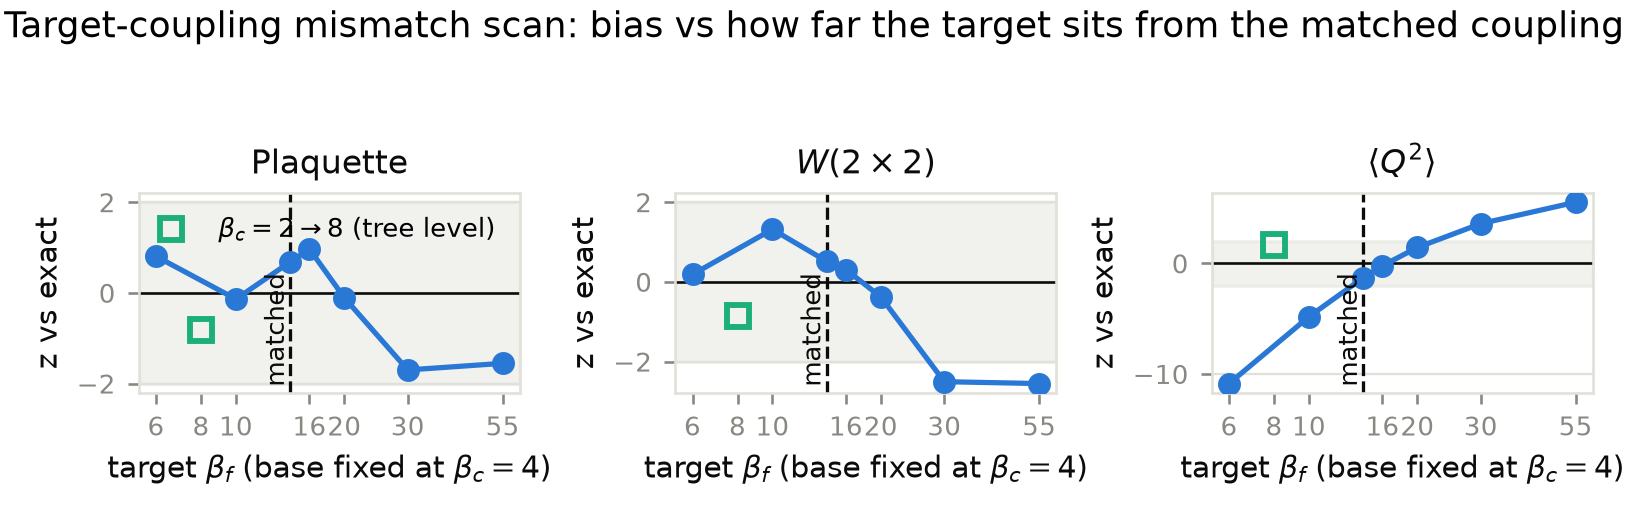
\includegraphics[width=0.9\linewidth]{figures/05_mismatch_scan.png}
  \caption{\textbf{Deliberate mismatch controls (part B).} The conditioning
  coarse ensemble is held at $\beta_c = 4$ while the target $\beta_f$ is
  varied off the matched value. The model tracks the \emph{requested}
  coupling --- evidence that $\beta$-conditioning, not the coarse input
  alone, sets the generated physics. Wilson observables pass; $P(Q)$, by
  design of the transport mode, remains the $\beta_c = 4$ base's sector
  histogram, which is \emph{structurally} wrong for the off-matched targets
  --- this track fails the exact-$P(Q)$ $\chi^2$ test under pure transport
  and is corrected by the exact-sector mode (Fig.~\ref{fig:mismatch-exact})
  or by a seconds-long instanton-HMC tail (Fig.~\ref{fig:pq-tail-mismatch}).}
  \label{fig:mismatch-transport}
\end{figure}

\begin{figure}[p]
  \centering
  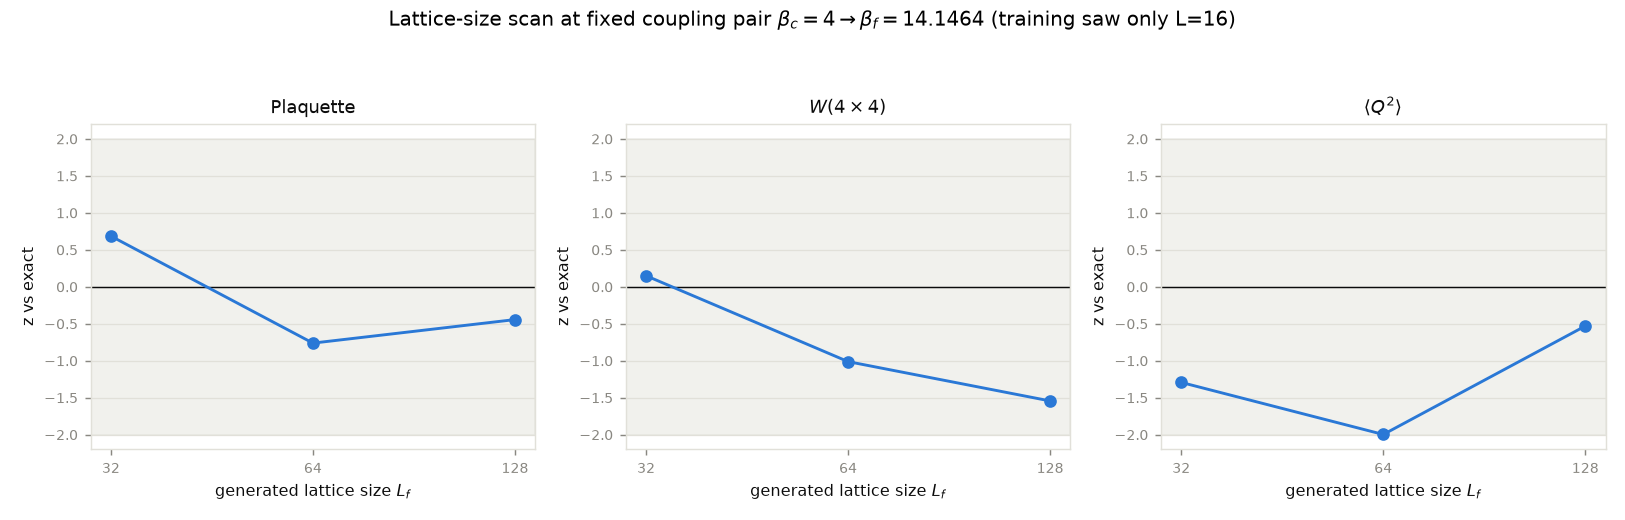
\includegraphics[width=0.9\linewidth]{figures/06_size_scan.png}
  \caption{\textbf{Volume transfer (part C).} The same checkpoint applied at
  $L = 64$ and $L = 128$ (never trained above $L = 32$); observables
  against exact values at $\beta_f = 14.15$. The v2 per-site normalization
  removes the lattice-size dependence that GroupNorm statistics introduced
  in earlier checkpoints.}
\end{figure}

\begin{figure}[p]
  \centering
  
\includegraphics[width=0.9\linewidth]{figures/07_raw_topology.png}
  \caption{\textbf{Raw (pre-enforcement) topology transport.} The
  model-level metric charge enforcement would otherwise hide: spurious raw
  $\langle Q^2 \rangle$ excess over the coarse base, per track. v2's
  symmetry augmentation (charge conjugation ties the $\pm Q$ sectors) cuts
  the mean excess from 5.3 (v6) to 2.9, with the largest gains at low
  $\beta$ (e.g.\ $+11.3 \to +1.5$) --- under the stricter no-$Q$-hop
  rethermalization.}
\end{figure}

\begin{figure}[p]
  \centering
  
\includegraphics[width=0.9\linewidth]{figures/08_case_low.png}
  \caption{\textbf{Representative low-$\beta$ case ($\beta_f = 3.10$,
  $L = 32$).} Full validation panel in the regime where topology fluctuates
  freely and HMC is healthy --- the pipeline must (and does) reproduce a
  broad $P(Q)$.}
\end{figure}

\begin{figure}[p]
  \centering
  
\includegraphics[width=0.9\linewidth]{figures/09_case_high.png}
  \caption{\textbf{Representative frozen-regime case ($\beta_f = 218.58$,
  $L = 32$).} Same panel deep in the topologically frozen regime (direct
  HMC: zero tunnelings). $\langle Q^2 \rangle$ agrees with the exact
  susceptibility; a fresh hot-start HMC ensemble at this coupling is wrong
  by two orders of magnitude in the same quantity.}
\end{figure}

\begin{figure}[p]
  \centering
  
\includegraphics[width=0.9\linewidth]{figures/10_case_extrapolation.png}
  \caption{\textbf{Extrapolation frontier ($\beta_f = 872.8$, $L = 32$).}
  Fifteen times the training maximum. Wilson observables pass against exact
  values. For topology, exact $\langle Q^2 \rangle \approx 9\cdot 10^{-4}$
  while every generated configuration has $Q = 0$: the sample variance of
  $Q^2$ is then exactly zero and the $z$-score is ill-defined (the verdict
  tables record it as $+\infty$ for this reason). The meaningful statement is
  that with expected nonzero-charge count $n\langle Q^2 \rangle \ll 1$ at this
  ensemble size, an all-zero sample is the modal outcome under the exact
  $P(Q)$ --- the sector content matches exact expectations rather than being
  merely ``consistent''.}
\end{figure}

\begin{figure}[p]
  \centering
  
\includegraphics[width=0.9\linewidth]{figures/11_case_L64.png}
  \caption{\textbf{Joint coupling + volume extrapolation
  ($\beta_f = 218.58$, $L = 64$).} The hardest case in the study: $4\times$
  the training coupling and $4\times$ the training area simultaneously.}
\end{figure}

\begin{figure}[p]
  \centering
  
\includegraphics[width=0.9\linewidth]{figures/12_timescales.png}
  \caption{\textbf{Thermalization timescales.} Per coupling: $t_{\rm therm}$
  of an HMC chain started from a raw diffusion sample (no rethermalization
  applied --- every sweep the seed needs is charged here), the equilibrated
  chain's own sampling interval $2\tau_{\rm int}$, and fresh hot/cold-start
  burn-in. Seeds thermalize in 0--13 trajectories in 26 of 29 cases (23 of 29 under
  the stricter below-$2	au_{
m int}$ criterion) ---
  below the interval, i.e.\ cheaper than the chain's marginal cost per
  config; fresh hot chains never thermalize above $\beta \approx 8.8$.}
\end{figure}

\begin{figure}[p]
  \centering
  
\includegraphics[width=0.9\linewidth]{figures/13_beta_scan.png}
  \caption{\textbf{Thermalization across the $\beta$ scan.} The same three
  quantities as a function of $\beta_f$: the ordering
  $t_{\rm therm}({\rm seed}) < 2\tau_{\rm int} < \text{burn-in(fresh)}$
  sets in at moderate coupling and widens as standard HMC slides into
  critical slowing down and topological freezing.}
\end{figure}

\begin{figure}[p]
  \centering
  
\includegraphics[width=0.9\linewidth]{figures/14_relaxation_mid.png}
  \caption{\textbf{Relaxation curves, $\beta_f = 55.02$ ($L = 32$).}
  Ensemble-mean observable traces for the three starting points with
  exponential fits and $|z| \le 2$ bands. The diffusion seed starts at its
  plateau (no measurable decay --- the desired outcome); hot and cold
  starts relax over hundreds of trajectories or not at all.}
\end{figure}

\begin{figure}[p]
  \centering
  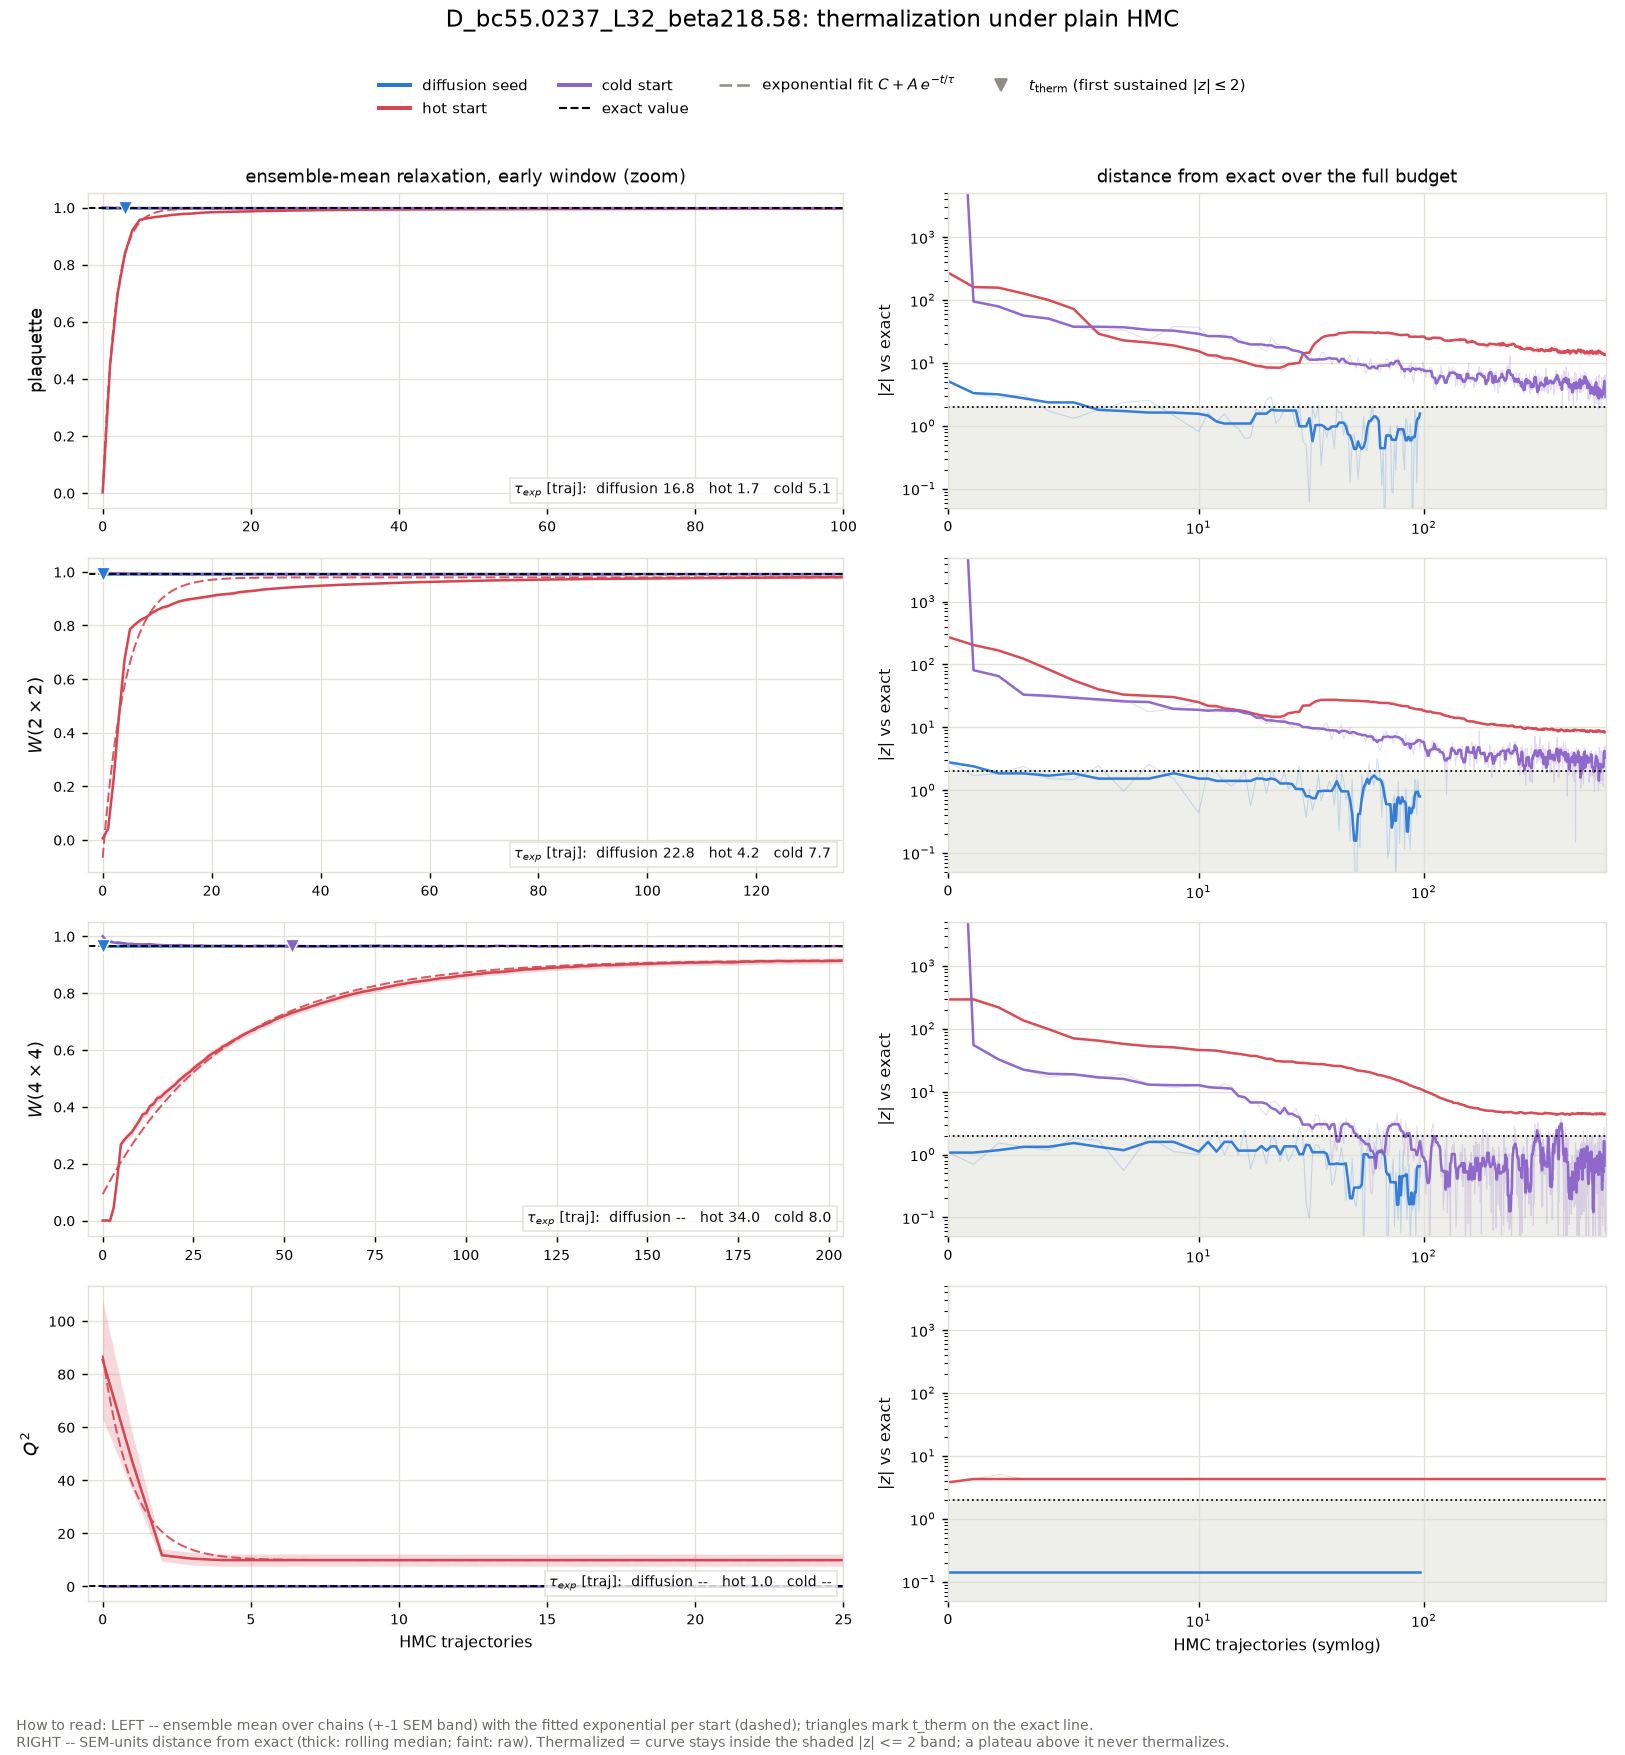
\includegraphics[width=0.9\linewidth]{figures/15_relaxation_high.png}
  \caption{\textbf{Relaxation curves, $\beta_f = 218.58$ ($L = 32$).} Same
  as the previous figure at the frozen regime's deep end: fresh chains
  never reach tolerance within the 640-trajectory budget; the seeded chain
  is indistinguishable from equilibrium within a few trajectories.}
\end{figure}

\begin{figure}[p]
  \centering
  
\includegraphics[width=0.9\linewidth]{figures/16_autocorrelation_modes.png}
  \caption{\textbf{Fast vs slow modes.} Normalized autocorrelation
  $\Gamma(\delta)$ of Wilson observables (fast modes) against the
  topological charge (slow mode) on equilibrated windows. Wilson-loop
  correlations decay within ${\sim}10$ trajectories while $\Gamma_Q$ stays
  pinned at 1 --- the frozen-topology signature; nothing in the seeded
  continuation depends on $Q$ mixing afterward, since the sector is
  transported, not evolved.}
\end{figure}

\begin{figure}[p]
  \centering
  
\includegraphics[width=0.85\linewidth]{figures/17_headtohead_cost.png}
  \caption{\textbf{Head-to-head vs instanton HMC: marginal cost and
  correctness ($L = 32$, burn-in 500, 128 configs/batch).} Instanton HMC
  --- the strongest classical baseline; its $Q$-hop keeps tunneling to
  $\beta = 256$ where standard HMC froze at 16 --- is far cheaper per
  config where it is correct (${\sim}0.01$\,s vs ${\sim}2.4$\,s), but open
  markers show it failing exactness (Wilson observables, up to $16.6\sigma$)
  at $\beta \ge 55$: its topology moves work, its UV does not thermalize.
  The diffusion pipeline passes everywhere at flat cost.}
  \label{fig:headtohead}
\end{figure}

\begin{figure}[p]
  \centering
  
\includegraphics[width=0.85\linewidth]{figures/18_entry_cost.png}
  \caption{\textbf{Entry cost vs $\beta$ --- the head-to-head's decisive
  plot.} Burn-in wall-clock required before the instanton-HMC ensemble
  agrees with exact results: 8\,s ($\beta = 4.4$), 16\,s ($\beta = 14.1$),
  1677\,s ($\beta = 55$, needing 8000 trajectories), and \emph{never within
  the tested budget} at $\beta = 218.58$ ($7.2\sigma$ off after 8000
  trajectories / 2534\,s). The baseline's entry cost grows
  ${\sim}200\times$ over one decade of $\beta$ and then stops converging.
  \textbf{The diffusion arm is charged its own entry cost here} (dashed
  line): the campaign that produced the checkpoint cost 8820\,s once
  (21.7\,min of HMC data generation plus 125.3\,min of training), which
  exceeds \emph{every} instanton-HMC burn-in that converges. For a single
  ensemble at a single coupling below $\beta \approx 55$, instanton HMC is
  cheaper outright. The generative cost is a fixed one-time charge plus a
  flat marginal cost (2.3--2.8\,s/config; amortized over the 38 study cases
  the campaign adds 1.8\,s/config, giving ${\sim}4.2$\,s/config), against a
  competitor cost that diverges with $\beta$. The claim this figure supports
  is therefore not ``diffusion is cheaper'' --- it is that the generative
  cost does not grow with $\beta$ while the baseline's does, and beyond
  $\beta \approx 55$ the baseline stops reaching correctness at any tested
  budget.}
  \label{fig:entry-cost}
\end{figure}

\begin{figure}[p]
  \centering
  
\includegraphics[width=0.85\linewidth]{figures/19_ess_weights.png}
  \caption{\textbf{Exact-likelihood diagnostic (honest negative).}
  Importance weights $w = e^{-S}/q$ from the probability-flow ODE
  likelihood (Hutchinson divergence, validated on an exactly solvable
  wrapped-Gaussian case), with the coarse-level density divided out via the
  matched-coupling action. The per-site weight spread is small
  (0.03--0.09 nats) but multiplies with volume, so ${\rm ESS}/N$ sits at
  the $1/N$ floor at $L = 32$ --- with the guidance term on or off,
  locating the gap in the score model's own density. The pipeline's
  correctness therefore rests on structural charge transport,
  rethermalization, and observable-level validation rather than
  reweighting; flow-based samplers with ${\rm ESS}/N \approx 0.5$--$0.7$
  hold that ground, while this pipeline's advantages are flat-cost seeding,
  extrapolation reach, and one-checkpoint generality. Closing the gap would
  require likelihood-aware training.}
\end{figure}

\begin{figure}[p]
  \centering
  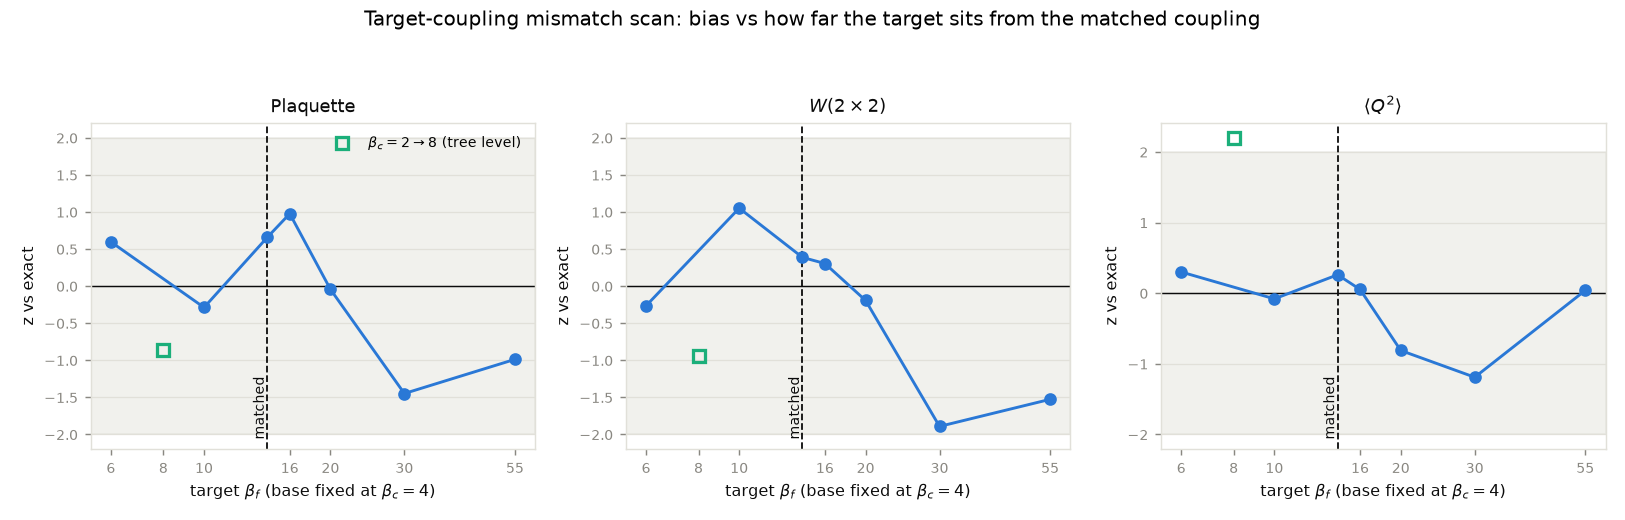
\includegraphics[width=0.9\linewidth]{figures/20_mismatch_exact_sectors.png}
  \caption{\textbf{Mismatch controls in exact-sector mode.} The part-B scan
  of Fig.~\ref{fig:mismatch-transport} rerun with C-antithetic base
  symmetrization and sectors resampled from the exact finite-volume $P(Q)$
  at each \emph{target} coupling. Every $\chi^2$ failure of the transport
  mode passes ($p = 0.0005 \to 0.43$ at $\beta_f = 6$;
  $0.0000 \to 0.94$ at 30; $0.005 \to 0.77$ at 55; $0.03 \to 0.32$ for the
  $\beta_c = 2 \to 8$ control; $0.005 \to 0.39$ at $L = 128$); Wilson
  observables are unchanged. Sector content is no longer inherited from the
  (deliberately wrong) base --- it is drawn where the target theory says it
  should be.}
  \label{fig:mismatch-exact}
\end{figure}

\begin{figure}[p]
  \centering
  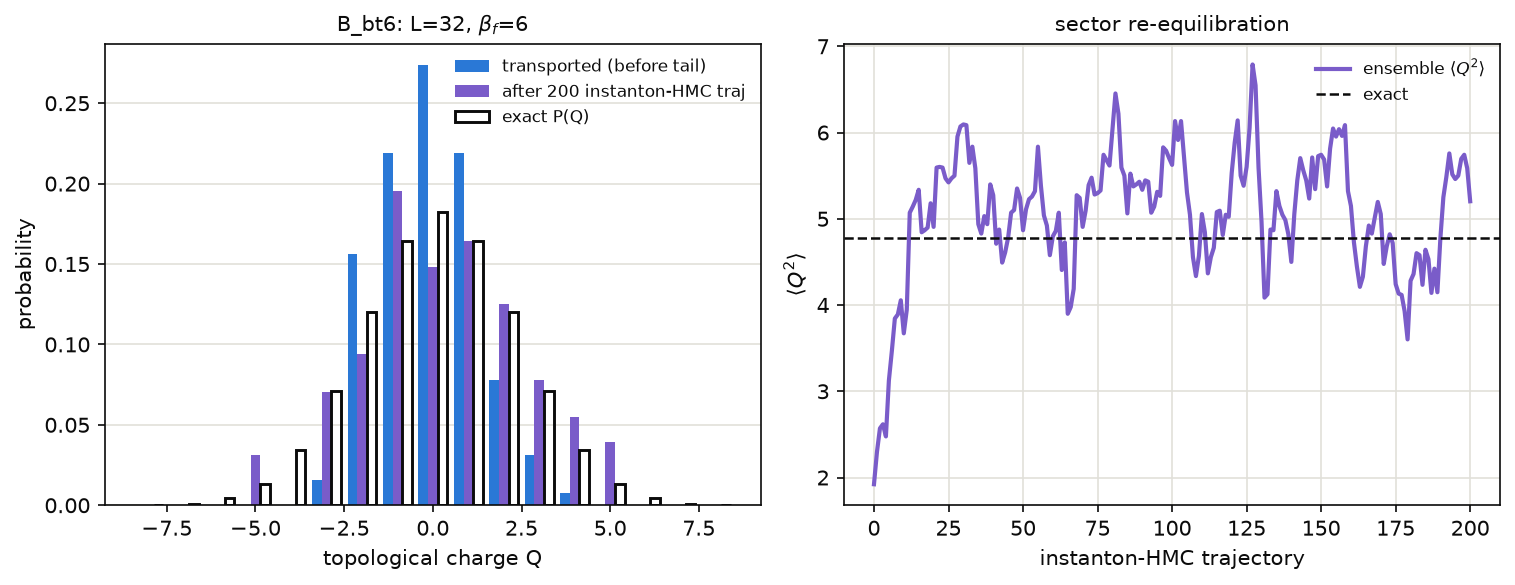
\includegraphics[width=0.9\linewidth]{figures/21_pq_tail_mismatch.png}
  \caption{\textbf{Sector re-equilibration by an instanton-HMC tail
  (B\_bt6, $L = 32$, $\beta_f = 6$).} The seeding claim, topologically:
  starting from the \emph{transported} ensemble --- whose $P(Q)$ is the
  mismatched $\beta_c = 4$ base's histogram, $\chi^2$ $p = 0.0005$ --- a
  200-trajectory HMC continuation with the instanton $Q$-hop restores
  $\langle Q^2 \rangle = 5.2$ vs exact 4.78 ($p = 0.39$) in 6 seconds of
  wall clock. Left: $P(Q)$ before/after vs exact; right: the
  $\langle Q^2 \rangle$ trajectory relaxing onto the exact line within tens
  of trajectories. The diffusion batch supplies the expensive part
  (thermalized UV at the target coupling); the topologically mixing tail is
  essentially free.}
  \label{fig:pq-tail-mismatch}
\end{figure}

\begin{figure}[p]
  \centering
  
\includegraphics[width=0.9\linewidth]{figures/22_pq_tail_L64.png}
  \caption{\textbf{Instanton-HMC tail at larger volume (C\_L64,
  $\beta_f = 14.15$, $L = 64$).} Same before/after construction on the
  size-scan rung: the tail moves the transported histogram onto the exact
  $P(Q)$ ($\chi^2$ $p$ $0.07 \to 0.70$) in 19 seconds, demonstrating the
  tail's cost stays trivial as the volume grows (the $Q$-hop's
  $\Delta S \approx 2\pi^2\beta/V$ is volume-independent).}
  \label{fig:pq-tail-L64}
\end{figure}

% -------------------------------------------------------------------

\begin{table}[p]
  \centering
  \caption{Instanton-HMC burn-in scan: entry cost vs quality at $L = 32$.
  Production window 640 trajectories $\times$ 32 chains throughout;
  quality = all Wilson-observable $|z| \le 2.5$ vs exact. Instanton-HMC
  $\langle Q^2 \rangle$ is correct in every row (the $Q$-hop works); the
  failures are UV thermalization.}
  \label{tab:burnin-scan}
  \begin{tabular}{rrrlrr}
    \toprule
    $\beta_f$ & burn-in & max Wilson $|z|$ & quality & entry cost (s) &
    diffusion s/config \\
    \midrule
    4.44   & 500  & 2.5  & pass & 8    & 2.28 \\
    14.15  & 500  & 1.7  & pass & 16   & 2.39 \\
    55.02  & 500  & 7.1  & fail & 31   & 2.37 \\
    55.02  & 2000 & 3.3  & fail & 328  & --   \\
    55.02  & 8000 & 1.1  & pass & 1677 & --   \\
    118.5  & 500  & 9.4  & fail & 42   & 2.76 \\
    218.58 & 500  & 16.6 & fail & 58   & 2.55 \\
    218.58 & 2000 & 7.8  & fail & 605  & --   \\
    218.58 & 8000 & 7.2  & fail & 2534 & --   \\
    \bottomrule
  \end{tabular}
\end{table}

\begin{table}[p]
  \centering
  \caption{Probability-flow ODE ESS of raw model transport. Guidance-off
  control: 0.019--0.021 at $L = 16$, 0.016 at $L = 32$ --- statistically
  identical, attributing the gap to the score model rather than the
  guidance terms.}
  \label{tab:ode-ess}
  \begin{tabular}{rrrr}
    \toprule
    $L$ & $\beta_f$ & ${\rm ESS}/N$ (fiber-corrected) &
    $\log w$ spread per site (nats) \\
    \midrule
    16 & 14.15  & 0.016 & 0.078 \\
    16 & 55.02  & 0.016 & 0.078 \\
    32 & 55.02  & 0.016 & 0.035 \\
    32 & 218.58 & 0.016 & 0.074 \\
    \bottomrule
  \end{tabular}
\end{table}

\begin{table}[p]
  \centering
  \caption{Sector-mode comparison over the 38-case study (same checkpoint
  and seeds). The exact-sector residuals are at the multiple-testing
  false-positive rate (${\approx}1.75$ expected at $\alpha = 0.05$ over 35
  tests); $\chi^2$ is computable for 35 of 38 cases --- the three
  deep-frozen cases (exact $\langle Q^2 \rangle \lesssim 10^{-3}$) have no
  populated bins to test.}
  \label{tab:sector-modes}
  \begin{tabular}{lrr}
    \toprule
    metric & transport & exact-sector \\
    \midrule
    exact-$P(Q)$ $\chi^2$ failures ($p < 0.05$) & 5/35 & 1/35 \\
    \quad of which mismatch track (B)           & 4    & 0    \\
    worst $|z(\langle Q^2 \rangle$ vs exact$)|$ & 11.8 & 2.8  \\
    cases with $|z(\langle Q^2 \rangle)| > 2$\textsuperscript{b} & 13 & 3 \\
    significant $\langle Q \rangle$ asymmetry ($|z| > 2$) & 0 & 0 \\
    mean plaquette $|z|$ vs reference (38 cases) & 1.77 & 1.74 \
    mean plaquette $|z|$ vs exact (38 cases)     & 1.06 & 1.08 \\
    \bottomrule
  \end{tabular}
\end{table}

\begin{table}[p]
  \centering
  \caption{$P(Q)$ before/after a 200-trajectory instanton-HMC tail, run on
  the transport-mode ensembles (the harder starting point). The
  frozen-regime row has too few populated $Q$ bins for a $\chi^2$ test; its
  $\langle Q^2 \rangle$ stays consistent with exact. All tails cost
  seconds --- negligible against either arm of the head-to-head in
  Table~\ref{tab:burnin-scan}.}
  \label{tab:pq-tail}
  \begin{tabular}{lrrrrrrrr}
    \toprule
    case & $L$ & $\beta_f$ & $\langle Q^2 \rangle$ before & after & exact &
    $\chi^2$ $p$ before & after & tail (s) \\
    \midrule
    B\_bt6      & 32 & 6      & 1.92  & 5.20  & 4.78  & 0.0005 & 0.39 & 6  \\
    A\_bc1.5    & 32 & 4.44   & 5.10  & 6.88  & 6.79  & 0.87   & 0.24 & 6  \\
    E\_bc11.8   & 32 & 43.6   & 0.44  & 0.54  & 0.58  & 0.31   & 0.96 & 16 \\
    D\_bc55.02  & 32 & 218.6  & 0.031 & 0.039 & 0.029 & --     & --   & 41 \\
    C\_L64      & 64 & 14.15  & 6.43  & 10.4  & 7.62  & 0.07   & 0.70 & 19 \\
    \bottomrule
  \end{tabular}
\end{table}

% ===================================================================
% Added 2026-08-03: brings this file level with appendix.md, which had
% advanced by one full revision (Figs 23-27, Tables S5-S7, the exactness
% endgame, and the scope/validation material below).
% ===================================================================

\subsection{Scope of the correctness claim}
\label{sec:appendix-v2-scope}

The deployed pipeline applies \textbf{no accept/reject step to the generated
proposal}: the only Metropolis moves are inside the local rethermalization
sweeps and the instanton $Q$-hop. Sixteen local sweeps \emph{reduce} the
proposal's bias; they do not remove it, and local updates relax
long-wavelength modes slowest. The generation pipeline is therefore a
\textbf{validated heuristic}, asymptotically exact only in the
rethermalization $\to \infty$ limit --- which costs what direct simulation
costs. Two claims are kept apart throughout:

\begin{itemize}
  \item \emph{Graded on observables} (this appendix's actual claim): the
    generated ensembles reproduce gauge-invariant observables against exact
    values to the precision quoted, including the residual bias quantified
    in Sec.~\ref{sec:appendix-v2-sharpness}.
  \item \emph{As a measure} (not claimed): the generated ensemble is
    demonstrably \emph{not} a sample from the target --- the measured density
    gap is ${\approx}1$ nat/site, i.e.\ 448 nats per configuration at
    $L = 16$, $\beta = 55$ and 2098 at $L = 32$, $\beta = 218.6$.
\end{itemize}

The conceptually exact mode is \emph{seeding}: an HMC chain started from a
diffusion configuration is asymptotically exact \emph{within its sector},
with the sector supplied by transport. That is the mode the head-to-head and
three-way results validate directly.

\paragraph{Why sector transport is exact, not approximate.} With
$\beta_f = 4\beta_c$ and $L_f = 2L_c$ the exact finite-volume
$\langle Q^2 \rangle \approx V/(4\pi^2\beta)$ is \emph{invariant} along the
ladder: for the Villain action the exact values over four rungs are
$1.20271 \to 1.20334 \to 1.20334 \to 1.20334$. The ladder multiplies $V$ and
$\beta$ by 4 simultaneously, so the coarse ensemble's $P(Q)$ \emph{is} the
fine theory's $P(Q)$ --- transport is an identity, not an approximation that
happens to work. Equivalently, climbing the ladder is a continuum-limit
trajectory at fixed physical volume: the endpoint ($L = 64$, $\beta = 55$)
is the same physical system resolved $8\times$ more finely than the base.
The campaign's measured-matching ladder inherits this to 4\%
($1.986 \to 1.934 \to 1.904 \to 1.903$), the drift sitting in the first,
strongest-coupling step where tree level is worst.

\subsection{Validation sharpness and the residual bias}
\label{sec:appendix-v2-sharpness}

The ``matches exact'' statement is an \emph{upper bound on bias}, and the
bound is tight: with $n = 64$--128 configs per case the median relative SEM
on $\langle \cos\theta_p \rangle$ is 0.0087\%, so $|z| > 2$ detects a
relative plaquette bias of \textbf{0.017\%} --- two parts in $10^4$. Three
residual features are visible at that precision (all computed on
$z_{\rm exact}$, which uses only the generated-ensemble error, the exact
value being noiseless):

\begin{itemize}
  \item \emph{A coherent negative offset.} All 20 Wilson-type observables
    have mean $z < 0$: plaquette $-0.423 \pm 0.204$ ($-2.1\sigma$),
    $W(2\times2)$ $-0.466 \pm 0.197$, $W(4\times4)$ $-0.436 \pm 0.177$. The
    generated ensembles are systematically very slightly \emph{less ordered}
    than exact.
  \item \emph{Over-dispersion.} $\mathrm{std}(z)$ should be 1 for a correct
    model with correct errors; measured, it is 1.255 (plaquette), 1.216
    ($W2{\times}2$), 1.316 ($W8{\times}8$), 1.438 ($W12{\times}12$), 2.785
    ($Q^2$). This is genuine case-to-case model bias, not an error-bar
    artifact: the coarse base delivered at thin${=}5$ has
    $\tau_{\rm int} = 0.50$--$0.62$ on every observable, bounding any
    inherited-correlation inflation at ${\le}1.12\times$.
  \item \emph{The bias concentrates in extended observables.}
    $\mathrm{std}(z)$ grows monotonically with loop area --- 1.093
    ($4{\times}4$), 1.226 ($6{\times}6$), 1.316 ($8{\times}8$), 1.339
    ($10{\times}10$), 1.438 ($12{\times}12$) --- with $\max|z|$ rising
    $3.12 \to 5.91$. Beyond-$3\sigma$ excursions over the \emph{full}
    observable set number 29 of 760 tests against 2.05 expected, versus 4 of
    114 over the $\{$plaquette, $W2{\times}2$, $W4{\times}4\}$ subset the
    case tables emphasize.
\end{itemize}

This is the observable-side shadow of the density gap: the residual model
error lives in long-wavelength modes, exactly the modes local
rethermalization relaxes slowest. Short-distance observables are reproduced
to $10^{-4}$; extended ones carry the error.

\subsection{The ESS-gap program}
\label{sec:appendix-v2-ess}

\begin{figure}[p]
  \centering
  
\includegraphics[width=0.85\linewidth]{figures/23_ess_progress.png}
  \caption{\textbf{The ESS-gap program across couplings.} Fiber-corrected
  log-weight spread measured with \emph{valid} weights (probability-flow ODE
  sampling returns each configuration with its own density; fresh seeds,
  $n = 64$), per checkpoint variant, absolute (left) and per site in nats
  (right). (i) The spread grows $\propto \beta V$ under the baseline: a
  small, nearly uniform per-plaquette density offset, not topology (sector
  action differences are $O(2\pi^2\beta/V) \approx 4$ nats against spreads of
  $10^2$--$10^3$) and not estimator noise. (ii) Both standard remedies go
  backwards: maximum-likelihood fine-tuning degrades every case despite
  improving its own validation metric, and single-case reverse-KL explodes
  the never-trained extrapolation coupling to ${\rm std} \approx 2202$.
  (iii) The guarded multi-case reverse-KL (rkl2) roughly halves the spread at
  \emph{every} case (16:55: $42 \to 19.7$; 32:218.6: $164 \to 103$),
  including the extrapolation monitor it never trained on. ESS$/N$
  nonetheless remains at the $1/N$ floor throughout.}
\end{figure}

\begin{figure}[p]
  \centering
  
\includegraphics[width=0.85\linewidth]{figures/24_proposal_sweep.png}
  \caption{\textbf{Sampling-time proposal sweep} (13 points, $L = 16$,
  $\beta_f = 55.02$). Every member of the proposal family yields valid
  weights, so ESS can be tuned with no retraining. The one free win:
  lowering the terminal noise floor ($\sigma_{\min}$ coefficient
  $0.1 \to 0.03$) takes the spread $27 \to 24$ and ESS$/N$
  $0.030 \to 0.031$. The clearest negative: \emph{strengthening} the
  exact-score blend monotonically worsens the density (blend 4:
  ${\rm std} = 128$), i.e.\ the harmonic $\beta_{\rm eff}$ approximation is a
  worse mid-$\sigma$ density than the learned score. Two stability controls
  (8 Hutchinson probes; 240 integration steps) sit at the baseline spread,
  pinning the spread on the model rather than the estimator.}
\end{figure}

\begin{figure}[p]
  \centering
  
\includegraphics[width=0.85\linewidth]{figures/25_finetune_dynamics.png}
  \caption{\textbf{Why the negative results are negative, and how the
  positive one was selected.} (a) The ML fine-tune (FFJORD-style,
  warm-started, 300 steps) raises held-out $\log q$/dof from $-0.887$ to
  $-0.520$ by step 75 (${\approx}190$ nats per configuration) yet its
  best-validation checkpoint \emph{worsens} deployed spread at every
  coupling: maximum likelihood raises the density on \emph{data}
  configurations, but the weights probe the density on the \emph{model's own
  samples}, making validation likelihood the wrong selection metric here.
  (b) The multi-case reverse-KL run internalizes that lesson: round-robin
  over three $(L,\beta)$ cases, evaluation on rotating disjoint coarse slices
  with rotating seeds, and checkpointing gated on mean training-case ESS
  improvement \emph{and} an extrapolation monitor ($L = 32$,
  $\beta = 218.6$, never trained on) staying below $1.5\times$ its initial
  spread. The guard blocked four of six save opportunities, including the
  step-100 state with the highest training ESS; the surviving step-250
  checkpoint is the one that generalized.}
\end{figure}

\begin{figure}[p]
  \centering
  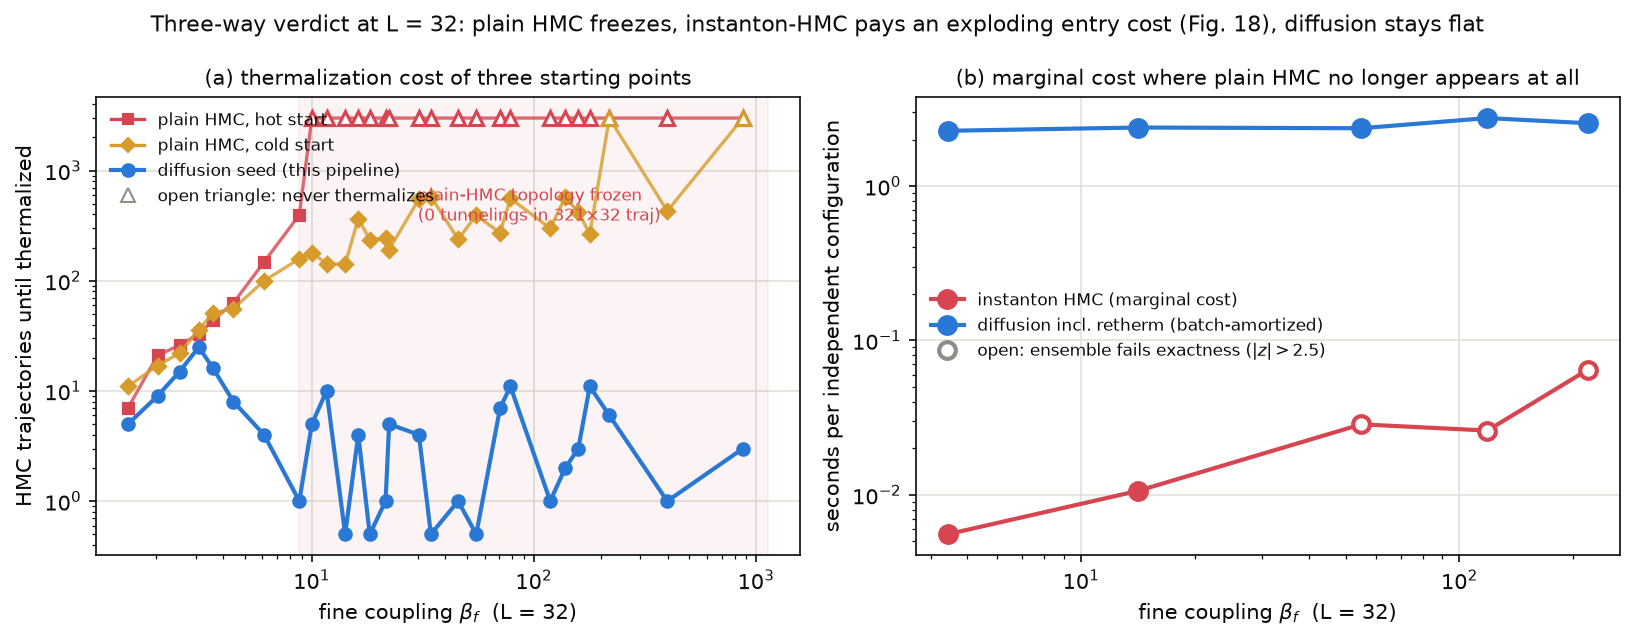
\includegraphics[width=0.85\linewidth]{figures/26_three_way.png}
  \caption{\textbf{The closing three-way verdict ($L = 32$).} (a) HMC
  trajectories until thermalization for three starting points across the
  matched-$\beta$ scan: hot-start plain HMC never thermalizes for
  $\beta \gtrsim 10$; cold-start needs hundreds of trajectories and its
  topology is frozen solid for $\beta \gtrsim 8.8$ (zero tunnelings in
  $321 \times 32$ trajectories, shaded region) --- so plain HMC produces
  ensembles whose $\langle Q^2 \rangle$ is silently wrong across the entire
  upper scan; a diffusion-generated seed thermalizes in 0--13 trajectories at
  every coupling to $\beta = 872.8$. (b) Marginal cost per independent
  configuration for the two survivors: instanton HMC is cheapest per
  configuration where it works, but its ensembles fail the exactness gates at
  $\beta \ge 55$ until the entry cost explodes, while the diffusion pipeline
  stays flat at ${\sim}2.4$\,s/config with filled (exact-agreeing) markers
  throughout.}
  \label{fig:three-way}
\end{figure}

\begin{figure}[p]
  \centering
  
\includegraphics[width=0.85\linewidth]{figures/27_program_optimum.png}
  \caption{\textbf{The ESS program at its measured optimum.} (a) Every
  model-quality intervention, chronological, at the reference case
  ($L = 16$, $\beta = 55$, fresh-seed verification): the $\sigma_{\min}$ knob
  and the guarded multi-case reverse-KL are the two keepers
  ($42 \to 24 \to 19.7$); ML fine-tuning, single-case reverse-KL, the
  $3.7\times$ capacity/data scale-up, and the 354-parameter correction head
  all went backwards and were discarded by the guard protocol. (b) The
  quantified end state: per-site density gap of the final checkpoint across
  the full $(L,\beta)$ plane --- 0.02--0.07 nats/site, uniformly 4--10$\times$
  above the ${\sim}0.005$ bar at which self-normalized weights would become
  usable.}
\end{figure}

\begin{table}[p]
  \centering
  \caption{ESS-gap program: fiber log-weight standard deviation by
  checkpoint variant. All rows are fresh-seed verification runs with valid
  weights (probability-flow ODE sampling, $n = 64$, 120 steps, 2 Hutchinson
  probes, $\sigma_{\min}$-coef 0.03 except the ladder-knobs row at 0.1).
  ESS$/N$ sits at or near the $1/64$ floor in every row except the knob-only
  point (0.031). Training cost of rkl2: 300 warm-started optimizer steps,
  ${\approx}80$ min on the laptop CPU; the campaign checkpoint itself is
  unmodified, and only this section's likelihood/ESS results use the
  fine-tuned variants.}
  \label{tab:ess-program}
  \begin{tabular}{lrrrr}
    \toprule
    variant & L16 $\beta$14.1 & L16 $\beta$55.0 & L32 $\beta$55.0 &
    L32 $\beta$218.6 \\
    \midrule
    v2 checkpoint, ladder knobs            & 17.9 & 42.1 & 84.3  & 163.7 \\
    v2 ckpt, $\sigma_{\min}$-coef 0.03     & ---  & 24.0 & ---   & ---   \\
    $+$ ML fine-tune (best-val, step 75)   & 29.0 & 41.3 & 131.8 & 293.6 \\
    $+$ single-case reverse-KL             & 23.9 & 24.1 & 75.1  & \textbf{2202} \\
    multi-case reverse-KL (rkl2, guarded)  & \textbf{15.1} & \textbf{19.7} &
      \textbf{40.8} & \textbf{102.6} \\
    big net (hidden 80, $+$24 L32 rungs)   & 19.7 & 31.6 & 49.6  & 211.9 \\
    \bottomrule
  \end{tabular}
\end{table}

\subsection{Exactness endgame: decomposition, AIS transport, $L = 64$}
\label{sec:appendix-v2-endgame}

\begin{table}[p]
  \centering
  \caption{Matching residual vs model error. Both arms blend-free at the
  \emph{trained} $\sigma$ floor (coef 0.3). $R^2_c$ is the fiber log-weight
  variance explained by coarse-only observables. The Villain arm was rerun on
  2026-08-03 after a bug fix: \texttt{approx\_matched\_coarse\_beta} had been
  called without its \texttt{action\_type} argument, so the arm ran at the
  \emph{Wilson}-matched $\beta_c$ (4.0, 14.1464) rather than the exact
  $\beta_f/4$ (3.5366, 13.7559). Both runs are internally valid; only the
  corrected one has the exact-matching property the control depends on.
  Correcting it made the Villain spreads \emph{larger} ($+4\%$, $+99\%$,
  $+51\%$) --- a train/test confound rather than a matching effect, since the
  checkpoint was trained on Wilson data at precisely the Wilson-matched
  couplings the buggy run used, so the corrected arm additionally pays an
  out-of-distribution conditioning penalty. The corrected Villain row is thus
  an \emph{upper bound} on model error and the subtraction
  Wilson${-}$Villain must not be read quantitatively.}
  \label{tab:matching-residual}
  \begin{tabular}{lrrr}
    \toprule
    arm & L16 $\beta$14.1 std/site ($R^2_c$) & L16 $\beta$55.0 &
    L32 $\beta$55.0 \\
    \midrule
    Wilson (matching residual $+$ model error) & 0.0209 (0.062) &
      0.0419 (0.005) & 0.0175 (0.023) \\
    Villain, $\beta_c = \beta_f/4$ exact (corrected) & 0.0298 (0.075) &
      0.0914 (0.003) & 0.0406 (0.077) \\
    Villain, Wilson-matched $\beta_c$ (superseded) & 0.0287 (0.174) &
      0.0459 (0.031) & 0.0268 (0.048) \\
    \bottomrule
  \end{tabular}
\end{table}

The conclusion survives on stronger, Villain-independent grounds. The matching
residual is by construction a function of the coarse configuration alone --- it
is the discrepancy between $S_{\rm matched}(c)$ and the true blocked action on
the same $c$ --- so it can contribute \emph{only} to the coarse-explainable
variance $R^2_c$. Wilson's $R^2_c$ is 0.062, 0.005, 0.023: at most ${\sim}6\%$
of the fiber log-weight variance is coarse-explainable at all, and that is
itself an upper bound because $c$-dependent \emph{model} error lands there
too. The matching floor is therefore negligible and the measured density gap
is fine-side model error, without needing the Villain arm at all; the Villain
comparison corroborates it (Wilson $\le$ Villain at every case, now by a wider
margin) without being load-bearing. The same decomposition run at the
\emph{deployment} settings (physics blend on, $\sigma_{\min}$-coef 0.03),
using the AIS stage's own samples, agrees independently:
$R^2_c = 0.003$--$0.064$ across the four cases.

\paragraph{Why the arm was not re-run against a Villain-trained checkpoint.}
The obvious repair --- train a Villain-specific model so the control arm is
free of the conditioning confound --- would replace one confound with a larger
one. It would compare \emph{two different checkpoints} (different capacity
utilization, training noise and seeds) rather than one checkpoint with and
without a matching residual. Table~\ref{tab:ess-program} measures how big that
substitution is: variants of the same architecture move fiber spreads by
factors of 2--6. The quantity being resolved here is bounded at a few percent
of the variance, an order of magnitude below the noise of any cross-model
comparison. No amount of retraining resolves an effect smaller than the
confound introduced to measure it, whereas the within-arm $R^2_c$
decomposition does and needs no second campaign. The study is therefore closed
with the corrected Villain numbers reported as-is, the confound named, and the
load-bearing argument moved to $R^2_c$.

\begin{table}[p]
  \centering
  \caption{AIS-corrected transport (final AIS result). Surrogate-bridge
  annealed importance sampling from ODE samples with exact initial density
  (48 bridge steps, 2 HMC $+$ instanton-hop updates per step; coefficients
  fit on the even half, quoted on the held-out odd half; 7-feature basis).
  The $R^2$ column is in-sample (refit on all data after CV ridge selection);
  with $n = 64$ and 6--11 predictors expect ${\sim}9$--17\% optimism, so the
  predicted floor is correspondingly optimistic. Held-out ESS$/N$ is at the
  $1/48$ floor in all four cases and should be read as ``at floor''.}
  \label{tab:ais-transport}
  \begin{tabular}{lrrrrr}
    \toprule
    case & std before & surrogate $R^2$ & predicted floor
    $\sqrt{1-R^2}\cdot$std & AIS std (held-out) & held-out ESS$/N$ \\
    \midrule
    16:14.1  & 17.0  & 0.717 & 9.0  & 30.6 & 0.021 \\
    16:55.0  & 17.6  & 0.332 & 14.4 & 18.6 & 0.024 \\
    32:55.0  & 36.4  & 0.664 & 21.1 & 28.4 & 0.021 \\
    32:218.6 & 117.5 & 0.839 & 47.1 & 44.7 & 0.021 \\
    \bottomrule
  \end{tabular}
\end{table}

The bridge saturates its theoretical floor where the gap is largest
(32:218.6: measured 44.7 vs predicted 47.1 --- a $2.6\times$ spread reduction
with the mechanism working exactly as derived), but held-out ESS$/N$ stays at
the $1/48$ floor everywhere: the weights degenerate on the topological-sector
component, which does not regress onto smooth features. A wider 11-feature
basis raised in-sample $R^2$ but exploded the held-out weights at 2 of 4
cases (std 1120 and 18{,}650). Recorded as the program's sixth honest
negative; the 7-feature run is the final AIS number and is now the code
default (\texttt{--basis final7}).

\paragraph{The measured KL.} For valid weights,
$E[\log w] - \Delta F_{\rm exact} = -{\rm KL}(q\|p)$ identically, with
$\Delta F$ exactly computable from the character expansion --- so the
free-energy certificate doubles as a direct measurement of the model's mean
density offset: ${\approx}0.88$ nats/site at 16:55 and 1.02 nats/site at
32:218.6. The structure of the remaining gap is therefore fully quantified: a
bulk smooth offset of ${\sim}1$ nat/site (mean), spread 0.02--0.07 nats/site
(variance), plus sector-frequency mismatch.

\paragraph{$L = 64$ head-to-head.} At $L = 64$, $\beta = 55$, the
instanton-HMC arm with the standard 400-trajectory burn-in fails every Wilson
observable at $z \approx +9$ to $+10$ while the diffusion arm passes all
observables (max $|z| = 1.83$, 8.6\,s/config including base, sampling and
retherm). The bias is positive (too ordered) and $Q^2$ is fine --- cold-start
relaxation of long-wavelength modes, not topology --- and it does \emph{not}
anneal away: max Wilson $|z| = 6.5$ at burn-in 1600 and 6.3 at 6400. The
competitor's marginal-cost advantage (0.036\,s per configuration, against the
diffusion arm's 8.6) is therefore purchased with an ensemble that is still
${\sim}6\sigma$ biased on Wilson observables after $16\times$ the standard
burn-in --- the entry-cost explosion of Fig.~18 materializing at scale,
measured rather than extrapolated.

\paragraph{Fresh-seed classification of the $3\sigma$ Wilson flags.} Four
cases in the campaign exceeded $3\sigma$ on a Wilson observable
(D\_bc14.1464, plaquette $-2.93$ and $W(2{\times}2)$ $-3.47$; B\_bt20,
$-3.19$; A\_bc8, $-2.71$; F\_L64, $W(2{\times}2)$ $+3.03$). Each was rerun
with two fresh seeds. Every mean-value flag flips sign or vanishes across
seeds --- D: $+2.24 / +2.97$ then $+0.45 / +0.57$; B: plaquette $-1.49$ then
$-0.04$, $W(2{\times}2)$ $-2.56$ then $+0.13$; A: $-1.33$ then $-0.02$;
F: $-0.86$ then $-1.28$ --- i.e.\ fluctuations, consistent with the ${\approx}0.2$
cases expected beyond $3\sigma$ over ${\sim}76$ tests. Two residuals are
recorded for completeness rather than dismissed. First, seed s3's A\_bc8
rerun shows $\langle Q^2\rangle$ $z = +4.18$ with exact-$P(Q)$ $\chi^2$
$p = 0.003$: a topology-transport excursion of the kind exact-sector mode is
built to remove (Table~\ref{tab:sector-modes}), not a Wilson-observable
failure. Second, F\_L64's minimum KS $p \approx 0.000$ in \emph{both} fresh
seeds --- a Wilson-loop \emph{distribution-shape} mismatch at the far
extrapolation whose means nonetheless pass. The latter is repeatable and is
therefore reported as a genuine residual defect of the far-extrapolation
regime, alongside the volume-growing raw $Q^2$ excess (1.7--2.7 at
$L \le 32$, rising to 7.1--28.2 at $L = 64$/128, rescued by exact-sector
mode). Provenance: \texttt{out/u1\_2d/generalization\_fresh\_s3/},
\texttt{\_s4/}.

\paragraph{Program closure.} The exactness program is closed at rkl2 $+$
$\sigma_{\min}$-coef 0.03 --- the measured optimum. The falsification chain
(sampling-time knobs, one win; data-side maximum-likelihood fine-tuning at
197k and at 354 parameters, both degrade deployment; single-case reverse-KL,
destroys extrapolation; guarded multi-case reverse-KL, the one $2\times$ win
then plateau; capacity/data scaling under DSM; per-level SMC restructuring;
and surrogate-bridge AIS) leaves the per-site density gap at 0.02--0.07
nats/site (spread) and ${\approx}1$ nat/site (mean) against the
${\sim}0.005$ usable-certificate bar. Exactness for this pipeline therefore
rests, by measurement rather than assumption, on the Markov-chain route ---
rethermalization, instanton-HMC tails, exact-sector resampling --- wrapped
around the generative proposal.

\subsection{Measuring the gap when ESS is uninformative}
\label{sec:appendix-v2-measuring}

The standard distributional check on a generative sampler is the
self-normalized effective sample size. It is the right instinct, and it fails
in exactly the regime one most needs it.

\paragraph{Why ESS stops reporting.} For self-normalized weights, ${\rm
ESS}/N$ is bounded below by $1/N$ --- the value taken when a single sample
carries all the weight. Every raw-transport case here sits at that bound
(Table~\ref{tab:ode-ess}: 0.016 with $N = 64$, i.e.\ $1/64$ to three digits).
That is not a small ESS; it is an \emph{unresolved} one. The estimator has
saturated and the true value could be arbitrarily smaller. Two proposals
whose log-weight spreads differ by an order of magnitude --- 15 nats and 164
nats, both present in Table~\ref{tab:ess-program} --- report the identical
${\rm ESS}/N$. Any program that tries to \emph{improve} a proposal while
monitoring ESS is therefore flying blind: the quantity it optimizes cannot
see the progress it makes. This is why the ESS-gap program is reported in
log-weight spread throughout, with ESS quoted only to confirm it never lifted
off.

\paragraph{What replaces it.} For weights that are valid --- meaning the
proposal density is known for the actual samples drawn --- the identity
\begin{equation}
  E_q[\log w] \;-\; \Delta F_{\rm exact} \;=\; -{\rm KL}(q \,\|\, p),
  \qquad
  w = \frac{e^{-S_f(x)}\, e^{+S_{\rm matched}(c)}}{q(x \mid c)},
\end{equation}
holds exactly. If $\Delta F$ can be computed independently, the \emph{mean}
log-weight is a direct measurement of the Kullback--Leibler divergence, in
nats. It is finite, it has a sem, and it is insensitive to how degenerate the
weights are: the mean of $\log w$ is well behaved precisely where the mean of
$w$ is not. That is what turns ``the weights are degenerate'' into ``the
density is off by 0.88 nats/site.''

Three ingredients are required, and each constrains where the method applies:

\begin{enumerate}
  \item \emph{Valid weights for the actual samples.} It is not enough to
    evaluate a density at a given configuration; the configurations must
    arrive with their own densities. Here the probability-flow ODE is
    \textbf{sampled}, accumulating the Hutchinson divergence along the same
    trajectory that produces the configuration, so each sample carries its
    exact $\log q$ in one pass. Evaluating a separately drawn ensemble under
    a discretized reverse map would \emph{not} give valid weights, because
    the evaluation map is not the inverse of the sampling map at finite step
    count.
  \item \emph{An independently computable $\Delta F$.} Supplied here by the
    character expansion of the 2D U(1) partition function on the torus. This
    ingredient does not transfer: without an exact free energy the identity
    still holds, but the KL cannot be read off and only the spread remains.
  \item \emph{Estimator control.} The Hutchinson trace estimator is unbiased
    in $\log q$ (it enters linearly); the residual concerns are
    discretization and probe noise. Both are bounded by explicit controls
    rather than assumed --- 8 probes and 240 integration steps each reproduce
    the baseline spread, pinning it on the model rather than the estimator.
\end{enumerate}

\paragraph{Validating the instrument.} Because the claim is a null result
about a model, the machinery is validated where the answer is known. On an
exactly solvable wrapped-Gaussian target with the true score and exact
divergence the pipeline returns ${\rm ESS}/N > 0.5$ --- it \emph{can} report
a healthy ESS, so the floor values above are a property of the model, not the
code. On synthetic exact weights the free-energy certificate closes to
$< 0.02$ nats. Both are unit tests.

\paragraph{Mean and variance are different diagnostics.} They are routinely
conflated under a single ESS number, and both are lost when it saturates. The
\textbf{mean} (the KL, ${\approx}1$ nat/site here) says how far the density
sits from the target on average --- a bulk offset, largely uniform per
plaquette. The \textbf{spread} (0.02--0.07 nats/site) says whether
reweighting is usable at all, since self-normalized estimators need total
spread of $O(1$--$3)$ before ESS lifts off. Reporting both makes the closure
quantitative: the residual is a ${\sim}1$ nat/site bulk offset plus a
0.02--0.07 nats/site spread plus sector-frequency mismatch, and it is the
\emph{spread}, not the mean, that keeps reweighting out of reach.

\paragraph{Separating model error from matching error.} One competing
explanation survives all of the above: the coarse conditioning ensemble is
drawn from a single-coupling action, whereas the true blocked measure of a
Wilson theory carries induced multi-coupling structure. The control is an arm
in which the matching is exact by construction --- the Villain action, where
blocking gives $\beta_c = \beta_f/4$ exactly --- so its spread is model error
alone. Wilson $\le$ Villain at every case, and Wilson's coarse-explainable
fraction sits \emph{below} Villain's model-error baseline
(Table~\ref{tab:matching-residual}): the matching floor is negligible and the
measured gap is fine-side model error, in full. This is what makes the
falsification chain a closure rather than an exhaustion, and it generalizes
--- any theory with an exactly-blockable companion action admits the same
control.

\subsection{A reporting protocol for learned coarse-to-fine samplers}
\label{sec:appendix-v2-protocol}

Everything above is specific to 2D U(1), but the failure mode is not: a
learned coarse-to-fine map can reproduce low-order gauge-invariant
observables to four significant figures while its density is off by ${\sim}1$
nat/site. That is what one should expect from a model trained on a local
objective and graded on a handful of low-dimensional projections; the physics
literature has an independent statement of the same hazard, namely that
Wilson loops decouple from the slow topological modes. The following is what
this study would have reported from the start.

\begin{enumerate}
  \item \textbf{Report the $z$-distribution, not a pass count.} ``38 of 38
    within $|z| \le 3$'' is compatible with a biased sampler and with
    underestimated errors, and distinguishes neither. Under a correct model
    with correct errors $z$ is standard normal across cases: report
    ${\rm mean}(z)$ and ${\rm std}(z)$. Here they are $-0.42$ and 1.26, both
    invisible in the pass counts.
  \item \textbf{Report dispersion against observable extent.} Short-distance
    agreement does not certify the measure. Here ${\rm std}(z)$ climbs
    monotonically $1.09 \to 1.44$ from $W(4\times4)$ to $W(12\times12)$;
    quoting only the plaquette and small loops hides the signal.
  \item \textbf{Eliminate the error-bar explanations before claiming model
    bias.} Measure $\tau_{\rm int}$ of the coarse base actually delivered to
    the model (0.50--0.62 here, bounding inflation at ${\le}1.12\times$), and
    state which error enters the quoted $z$ --- against an \emph{exact} value
    only the generated ensemble's error enters, so a reference chain's
    autocorrelation cannot inflate it.
  \item \textbf{Do not report a saturated ESS as a number.} If ${\rm ESS}/N$
    equals $1/N$ to the digits shown, say ``degenerate'' and report the
    log-weight spread instead.
  \item \textbf{Where an exact free energy exists, report the KL directly},
    with mean and spread quoted separately.
  \item \textbf{Include an exactly-matched control arm} to separate matching
    error from model error; without it a list of failed remedies is
    exhaustion, not a result.
  \item \textbf{State the multiplicity, and apply it symmetrically.} Reruns
    of flagged cases with fresh seeds should be accompanied by reruns of a
    matched sample of unflagged cases; otherwise regression to the mean
    guarantees the flags vanish.
  \item \textbf{Charge the generative arm its entry cost.} Quote the one-time
    cost, the marginal cost, and the break-even configuration count. Here the
    one-time cost (8820\,s) exceeds every classical burn-in that converges,
    and the defensible claim is about \emph{scaling}, not about being
    cheaper.
  \item \textbf{Report raw, pre-enforcement topology.} Any structural sector
    imposition makes the final histogram correct by construction; the
    informative numbers are the raw charge-match rate (0.21) and the raw
    $\langle Q^2 \rangle$ excess, which \emph{grows with volume} (1.7--2.7 at
    $L \le 32$ to 7.1--28.2 at $L = 64/128$). Be explicit about which
    mechanism supplies the difference and whether it exists in the target
    theory.
  \item \textbf{Say which mode the correctness claim attaches to.} A
    generation pipeline with no accept/reject on the proposal is a heuristic
    validated on observables; a seeded chain run with an exact kernel is
    asymptotically exact. Conflating them is the easiest way for an honest
    study to overclaim.
\end{enumerate}
